\section{Planar boundaries and finite scales}\label{sec:preliminaries}

We now fix either the bond or the site model. This section supplies a planar
boundary count and chooses all the finite scales needed to lower the parameter.
The boundary count will be used first to show $p_c<1$, and then to prove that
the adaptive exploration survives.

\subsection{A deterministic boundary count}

An edge of the dual square lattice
$\mathbb Z^2+(1/2,1/2)$ crosses exactly one primal edge of $\mathbb Z^2$.
For a finite set $X\subset\mathbb Z^2$, its dual edge boundary consists of
the dual edges crossing primal edges with exactly one endpoint in $X$.

\begin{lemma}[Boundary cycles]\label{prelim:contours}
There are deterministic families $\mathcal C_n$ of simple dual cycles of
length $n$, with $|\mathcal C_n|\le 2n3^n$, such that the dual edge boundary
of every finite $X\subset\mathbb Z^2$ containing $0$ includes a cycle in
$\bigcup_{n\ge1}\mathcal C_n$. For each cycle in $\mathcal C_n$, one can
fix at least $n/7$ of its crossed primal edges with pairwise disjoint endpoints.
\end{lemma}

\begin{proof}
At a dual vertex, the boundary degree counts the membership changes around
a primal square, and is therefore even. The finite dual boundary consequently
decomposes into edge-disjoint simple cycles: extract a simple cycle whenever
an edge remains, and remove its edges, preserving even degrees.

Along the positive horizontal ray from $0$, the total number of boundary
crossings is odd, since membership in $X$ starts at one and eventually becomes
zero. At least one cycle in the decomposition has an odd number of positive-ray
crossings. The total number of crossings of a closed dual cycle with the whole
horizontal line is even, by counting changes of the sign of the height.
The selected cycle therefore also crosses the negative ray.

If its length is $n$, a positive crossing has horizontal coordinate
$t+1/2$ for some integer $0\le t<n$: the horizontal distance to a negative
crossing is less than $n$. Define $\mathcal C_n$ to be all simple length-$n$
cycles having such an anchored crossing and an odd number of positive-ray
crossings. There are at most $n$ choices for the anchored edge, two orientations,
and at most $3^n$ nonbacktracking continuations. This proves the asserted
overcount. Finally, greedily select crossed primal edges in a fixed order,
discarding all edges incident to either endpoint of each selection. Each
selection discards at most seven edges, including itself, because the primal
degree is four. The selected edges have disjoint endpoints and number at least
$n/7$.
\end{proof}

\begin{lemma}\label{prelim:pc-below-one}
For both models on $\mathbb Z^3$, $p_c<1$.
\end{lemma}

\begin{proof}
It suffices to percolate on a coordinate copy of $\mathbb Z^2$. In the bond
model, if the origin cluster there is finite, all primal edges crossed by its
dual boundary are closed. Lemma~\ref{prelim:contours} and a union bound give
\[
 \mathbb P_p(0\text{ has a finite planar cluster})
 \le \sum_{n\ge1}2n3^n(1-p)^n<1
\]
for $p<1$ sufficiently close to one.

For sites, first separate the event that $0$ is closed. If its open planar
cluster is finite, each edge crossed by the boundary cycle has a closed
endpoint. For a fixed candidate cycle, select $k\ge n/7$ edges with disjoint
endpoints as in Lemma~\ref{prelim:contours}. The union over choices of one
closed endpoint of each edge has probability at most $[2(1-p)]^k$.
For $p$ close to one, $2(1-p)<1$, so
\[
 \mathbb P_p(0\text{ is not in an infinite planar open cluster})
 \le (1-p)+\sum_{n\ge1}2n3^n[2(1-p)]^{n/7}<1.
\]
Indeed both displayed series are convergent geometric-power series tending
to zero as $p\uparrow1$. This proves the lemma.
\end{proof}

\subsection{Seed boxes and quarter-faces}

For $u\in\mathbb Z^3$ and a nonnegative integer $b$, write
\[
 \Lambda_b(u)=u+([-b,b]^3\cap\mathbb Z^3),\qquad \Lambda_b=\Lambda_b(0).
\]
A \emph{quarter-face} of $\Lambda_b(u)$ is obtained by setting one coordinate
relative to $u$ equal to $b$ or $-b$, and restricting each remaining coordinate
to either $[0,b]$ or $[-b,0]$. There are 24 such quarter-faces; overlaps on their
boundaries do not matter. More explicitly, for a normal index
$i\in\{1,2,3\}$, a sign $\sigma\in\{-1,+1\}$, and signs
$\varepsilon_j\in\{-1,+1\}$ for the two indices $j\ne i$, set
\begin{equation}\label{prelim:face-index}
 F_{i,\sigma}^{(\varepsilon_j)_{j\ne i}}(u,b)
 =\{u+x:x_i=\sigma b,\quad
                  0\le\varepsilon_jx_j\le b\ (j\ne i)\}.
\end{equation}
The six choices of $(i,\sigma)$ and the four choices of the transverse
sign pair enumerate all 24 faces. Figure~\ref{prelim:quarterfaces-figure}
illustrates this indexing.
A bit is \emph{internal} to a vertex set if it is a
site in that set, or, for bonds, an edge with both endpoints in that set.

\begin{figure}[tbp]
\centering
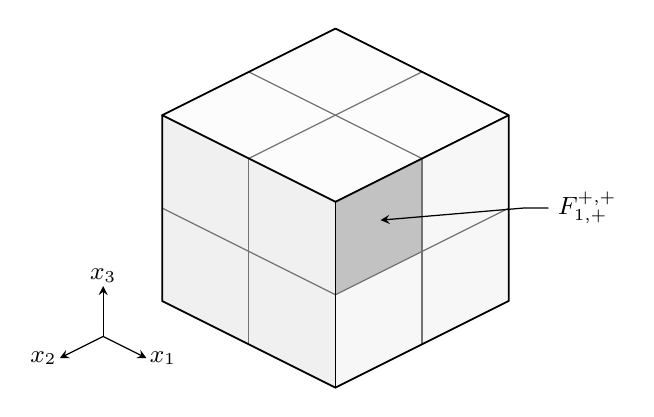
\begin{tikzpicture}[
  x={(1.10cm,-0.55cm)},
  y={(-1.10cm,-0.55cm)},
  z={(0cm,1.18cm)},
  font=\small,
  line join=round,
  line cap=round,
  >=stealth,
  qf edge/.style={black,line width=0.65pt},
  qf division/.style={black!55,line width=0.45pt}
]
  \fill[black!3] (1,-1,-1)--(1,1,-1)--(1,1,1)--(1,-1,1)--cycle;
  \fill[black!6] (-1,1,-1)--(1,1,-1)--(1,1,1)--(-1,1,1)--cycle;
  \fill[black!1] (-1,-1,1)--(1,-1,1)--(1,1,1)--(-1,1,1)--cycle;

  \fill[black!24] (1,0,0)--(1,1,0)--(1,1,1)--(1,0,1)--cycle;

  \draw[qf division] (1,0,-1)--(1,0,1);
  \draw[qf division] (1,-1,0)--(1,1,0);
  \draw[qf division] (0,1,-1)--(0,1,1);
  \draw[qf division] (-1,1,0)--(1,1,0);
  \draw[qf division] (0,-1,1)--(0,1,1);
  \draw[qf division] (-1,0,1)--(1,0,1);

  \draw[qf edge]
    (1,-1,-1)--(1,1,-1)--(-1,1,-1)--(-1,1,1)
    --(-1,-1,1)--(1,-1,1)--cycle;
  \draw[qf edge] (1,1,1)--(1,1,-1);
  \draw[qf edge] (1,1,1)--(-1,1,1);
  \draw[qf edge] (1,1,1)--(1,-1,1);

  \coordinate (qf representative) at (1,0.48,0.56);
  \begin{scope}[x=1cm,y=1cm]
    \node[anchor=west] (qf label) at (2.70,0.00) {$F_{1,+}^{+,+}$};
    \draw[->,line width=0.45pt]
      (qf label.west)--(2.38,0.00)--(qf representative);

    \coordinate (qf axes) at (-2.95,-1.63);
    \draw[->,line width=0.45pt]
      (qf axes)--(-2.40,-1.905) node[right,inner sep=1pt] {$x_1$};
    \draw[->,line width=0.45pt]
      (qf axes)--(-3.50,-1.905) node[left,inner sep=1pt] {$x_2$};
    \draw[->,line width=0.45pt]
      (qf axes)--(-2.95,-0.99) node[above,inner sep=1pt] {$x_3$};
  \end{scope}
\end{tikzpicture}
\caption{Quarter-faces of $\Lambda_b(u)$, shown schematically for $b>0$.
Each of the three visible faces is divided into four quarter-faces;
the three opposite faces are divided in the same way.
Thus $3$ normal axes $\times\,2$ normal signs $\times\,4$ transverse sign pairs
give $24$ quarter-faces. Boundary overlaps are permitted.
The shaded example $F_{1,+}^{+,+}$ has $x_1-u_1=b$ and
$0\le x_2-u_2,x_3-u_3\le b$.}
\label{prelim:quarterfaces-figure}

\end{figure}

Suppose, towards a contradiction, that at $p=p_c$ an infinite cluster exists
with positive probability. Then $0<p<1$ by Lemma~\ref{prelim:pc-below-one}
and the absence of percolation at zero. In fact an infinite cluster exists
almost surely. To see this without a uniqueness assumption, the existence event
is invariant under changing finitely many bits. Deleting finitely many edges,
or finitely many vertices in a locally finite graph, splits an infinite
connected component into only finitely many components, at least one of which
is infinite. The event is measurable by countably many finite-path tests, and
is determined by the bits outside any finite set. Thus it is independent of
every finite cylinder event. Finite cylinder events approximate all events
in this countable product space in probability, so the existence event is
independent of itself and has probability zero or one.
It follows that
\begin{equation}\label{prelim:seed-infinite}
 \mathbb P_p(\Lambda_m\text{ meets an infinite cluster})\longrightarrow1
 \qquad(m\longrightarrow\infty).
\end{equation}

We also use Harris's positive-association inequality~\cite{Harris1960}
for increasing events under a finite product
of independent bits, and of decreasing events. Here is an elementary proof.
For two increasing functions, condition on the last bit. Induction bounds the
conditional covariance below by zero. The conditional means are increasing
functions of this last bit, whose covariance is nonnegative. The covariance
decomposition proves the assertion by induction on the number of bits.
The same argument works for decreasing functions, and iteration gives the
intersection bound for any finite family of events.

The use of symmetric quarter-face estimates follows the renormalization
framework of Kozma and Nitzan~\cite[Section~4, Lemmas~8--9]{KozmaNitzan2024}.
The next lemma fixes the geometry before decreasing $p$. Its tolerance $f$
is reserved for the planar contour sum, while $\gamma$ bounds the probability
of missing one quarter-face. The intermediate tolerances distribute errors
in the extension and exploration arguments. Once all scales have been chosen
at $p$, finite-event continuity will supply one $q<p$ for the three required
radii.

\begin{lemma}[Choice of scales]\label{prelim:scales}
Under the preceding contradiction assumption, there are numbers
$f,\delta,\eta,\tau,\gamma\in(0,1)$, positive integers $m,K,R,r$, and
$q\in(p/2,p)$ with the following properties. First, $f<1/2$ and
\begin{equation}\label{prelim:contour-budget}
 \sum_{n\ge1}2n3^n(2f)^{n/7}<1.
\end{equation}
The error parameters satisfy
\begin{equation}\label{prelim:budgets}
 \delta+\frac{52\eta}{\delta}<f,\qquad
 \tau<\frac\eta4,\qquad \gamma<\delta,\qquad
 \frac{2\gamma}{\tau}<\frac\eta4.
\end{equation}
Let $M$ be the number of internal bits of $\Lambda_m$, and set
$\rho_0=(p/2)^{M+1}$. With $L=K(8m+5)^3$ and $\alpha=(1-p)^L$, we have
\begin{equation}\label{prelim:scale-inequalities}
 \frac4{K\rho_0}<\frac\eta4,\qquad
 R>m,\qquad \frac1{\alpha(R-m)}<\frac\eta4,\qquad r>100(R+1).
\end{equation}
For every $\ell\in\{2r,2r+1,10r\}$, $u\in\mathbb Z^3$, and quarter-face
$F$ of $\Lambda_\ell(u)$, independent parameter-$q$ percolation satisfies
\begin{equation}\label{prelim:quarterface}
 \mathbb P_q\bigl(\Lambda_m(u)\leftrightarrow F
              \text{ within }\Lambda_\ell(u)\bigr)>1-\gamma.
\end{equation}
\end{lemma}

\begin{proof}
The series in \eqref{prelim:contour-budget} tends to zero as $f\downarrow0$,
so choose $f$ first. Choose $\delta<f$, then $\eta$ sufficiently small for
the first inequality of \eqref{prelim:budgets}, then $\tau$, and finally
$\gamma$, in that order. By \eqref{prelim:seed-infinite}, choose $m\ge1$
so that the probability that $\Lambda_m$ meets no infinite cluster at
parameter $p$ is less than $(\gamma/2)^{24}$.

For every integer $\ell>m$, any infinite cluster meeting $\Lambda_m$
gives an open path from $\Lambda_m$ to the vertex boundary of $\Lambda_\ell$
inside that cube. Thus the probability of missing the whole boundary is less
than $(\gamma/2)^{24}$. By signed coordinate symmetry, all 24 quarter-face
miss events have the same probability, say $a_\ell$. They are decreasing
events of a finite product, so positive association gives
\[
 a_\ell^{24}\le
 \mathbb P_p(\Lambda_m\text{ misses every quarter-face within }\Lambda_\ell)
 <(\gamma/2)^{24}.
\]
Consequently $a_\ell<\gamma/2$ for every $\ell>m$.

Now $M$ and $\rho_0$ are fixed and positive. Choose $K$, define $L$ and
$\alpha>0$, and choose $R$ and then $r$ to satisfy
\eqref{prelim:scale-inequalities}. All these choices precede the choice of
$q$. At each of the three radii $2r,2r+1,10r$, a quarter-face connection
event uses finitely many bits, so its probability is a polynomial in the
parameter. The strict estimate at $p$, with margin $\gamma/2$, therefore
persists with margin $\gamma$ at some single $q\in(p/2,p)$, simultaneously
for all 24 faces and all three radii. Translation invariance gives the same
estimates for every center $u$. This proves \eqref{prelim:quarterface}.
\end{proof}

Fix these choices for the rest of the proof. Every later connection estimate
uses parameter $q$ on the indicated unrevealed region. Bits outside that region
may already have been fixed, a possibility allowed by
Corollary~\ref{cmp:failure}.
